\chapter{Modelling}%
\label{ch:modelling}

\section{Finger model}%
\label{sec:finger_model}

For modelling the finger, we're assuming that the motion is limited to a 2D-plane. This is mostly true, due to the collateral ligaments at the DIP- and the PIP-joint, preventing excessive side-to-side bending, as discussed in \cref{subsec:theory_hand_anatomy}. The MCP joint doesn't have the same support-structure, so it's free to move side to side, but this isn't as relevant to model for the task at hand, as the lateral movement from the cable pulling on the finger is minimal.

For our model, we assume that the finger is composed of three links, with three revolute joints, like a \textit{planar manipulator} \parencite{PlanarManipulatorOverview}. To model the stiffness from the tendons and ligaments, we'll add a torsional spring at each joint. The springs will have a non-zero equilibrium angle, representing the natural resting position of the finger joints. The damping from the soft tissue will be modeled by torsional dampers. A schematic of the model can be seen in \cref{fig:modelling_finger_model}. We'll model the links as rigid cylinders, with uniform mass distribution, and the joints as ideal revolute joints, with no friction. The parameters of the model are listed in \cref{tab:finger_params}.

\begin{figure}
    \centering
    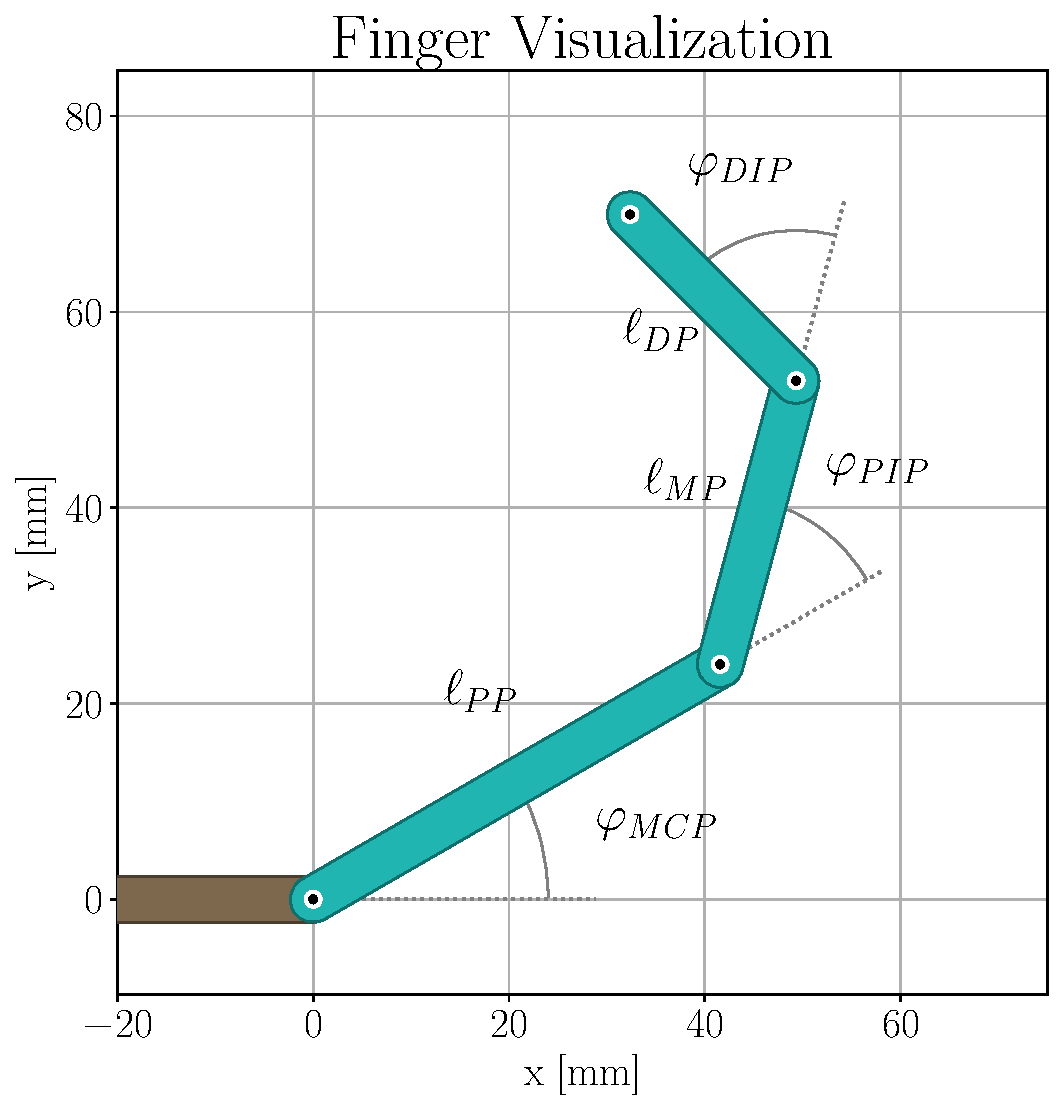
\includegraphics[width=1.0\textwidth]{../Figures/Modelling/finger_variables_visualization.pdf}
    \caption{Visualization of the finger model, with three revolute joints, where the relative joint angles, and the lengths of each phalanx are labeled.}
    \label{fig:modelling_finger_model}
\end{figure}

\begin{table}
    \caption{Parameters used in the finger model.}
    \label{tab:finger_params}
    \centering
    \begin{tabular}{llccc}
        \toprule
        Parameter & Link/joint & Symbol & Value & Unit \\
        \midrule
        \multirow{3}{*}{Mass}
            & PP & $m_{\jnt{PP}}$ & $20$ & \multirow{3}{*}{$\si{\gram}$} \\
            & MP & $m_{\jnt{MP}}$ & $15$ & \\
            & DP & $m_{\jnt{DP}}$ & $20$ & \\
        \midrule
        \multirow{3}{*}{Length}
            & PP & $l_{\jnt{PP}}$ & $48$ & \multirow{3}{*}{$\si{\milli\metre}$} \\
            & MP & $l_{\jnt{MP}}$ & $30$ & \\
            & DP & $l_{\jnt{DP}}$ & $24$ & \\
        \midrule
        \multirow{3}{*}{Radius}
            & PP & $r_{\jnt{PP}}$ & $8.5$ & \multirow{3}{*}{$\si{\milli\metre}$} \\
            & MP & $r_{\jnt{MP}}$ & $8.5$ & \\
            & DP & $r_{\jnt{DP}}$ & $8.5$ & \\
        \midrule
        \multirow{3}{*}{Equilibrium angle}
            & MCP & $\varphi_{\jnt{MCP, eq}}$ & $\pi/6$ & \multirow{3}{*}{$\si{\radian}$} \\
            & PIP & $\varphi_{\jnt{PIP, eq}}$ & $\pi/4$ & \\
            & DIP & $\varphi_{\jnt{DIP, eq}}$ & $\pi/12$ & \\
        \midrule
        \multirow{3}{*}{Stiffness coefficient}
            & MCP & $k_{\jnt{MCP}}$ & $0.5$ & \multirow{3}{*}{$\si{\newton\metre\per\radian}$} \\
            & PIP & $k_{\jnt{PIP}}$ & $0.5$ & \\
            & DIP & $k_{\jnt{DIP}}$ & $0.5$ & \\
        \midrule
        \multirow{3}{*}{Damping coefficient}
            & MCP & $b_{\jnt{MCP}}$ & $0.05$ & \multirow{3}{*}{$\si{\newton\metre\second\per\radian}$} \\
            & PIP & $b_{\jnt{PIP}}$ & $0.05$ & \\
            & DIP & $b_{\jnt{DIP}}$ & $0.05$ & \\
        \bottomrule
    \end{tabular}
\end{table}

To model the dynamics of the finger, we'll use the Euler-Lagrange equations as shown in \cref{subsec:theory_modelling_euler_lagrange_equations}. We'll define our generalized coordinates as the relative joint angles, $\varphi_{\jnt{MCP}}$, $\varphi_{\jnt{PIP}}$ and $\varphi_{\jnt{DIP}}$:

\begin{equation}
    \label{eq:modelling_finger_generalized_coordinates}
    \mathbf{q} \triangleq \begin{bmatrix}
        \varphi_{\jnt{MCP}} \\
        \varphi_{\jnt{PIP}} \\
        \varphi_{\jnt{DIP}}
    \end{bmatrix}
    \Longrightarrow
    \dot{\mathbf{q}} = \begin{bmatrix}
        \dot{\varphi}_{\jnt{MCP}} \\
        \dot{\varphi}_{\jnt{PIP}} \\
        \dot{\varphi}_{\jnt{DIP}}
    \end{bmatrix}
    \Longrightarrow
    \ddot{\mathbf{q}} = \begin{bmatrix}
        \ddot{\varphi}_{\jnt{MCP}} \\
        \ddot{\varphi}_{\jnt{PIP}} \\
        \ddot{\varphi}_{\jnt{DIP}}
    \end{bmatrix}.
\end{equation}

To derive the equations of motion, we need to define the kinetic energy, $T$, and the potential energy, $V$ of our system. 

\subsection{Kinetic energy}
The kinetic energy will be the sum of the kinetic energy of each link, which can be decomposed into the rotational and translational kinetic energy, defined as:

\begin{equation}
    \label{eq:modelling_kinetic_energy_total}
    T_{\text{tot}} = T_{\text{rot}} + T_{\text{trans}}.
\end{equation}

\subsection*{Rotational kinetic energy}

The rotational kinetic energy of the system is rather straightforward to derive, as the angular velocity of each link is equal to the time derivative of the joint angle. Since the angles are relative, the total angular velocity of each link is the sum of the time derivatives of the joint angles up to that link. Hence, the rotational kinetic energy can be expressed as:

\begin{equation}
    \label{eq:modelling_rot_kinetic_energy}
    T_{\text{rot}} = \frac{1}{2}J_{\jnt{MCP}}\dot{\varphi}_{\jnt{MCP}}^2 + \frac{1}{2}J_{\jnt{PIP}}(\dot{\varphi}_{\jnt{MCP}} + \dot{\varphi}_{\jnt{PIP}})^2 + \frac{1}{2}J_{\jnt{DIP}}(\dot{\varphi}_{\jnt{MCP}} + \dot{\varphi}_{\jnt{PIP}} + \dot{\varphi}_{\jnt{DIP}})^2.
\end{equation}

\subsection*{Translational kinetic energy}

The translational kinetic energy is a bit more complex to derive, as the linear velocity of each link depends on the geometry of the system. The linear velocity of each link can be derived by finding the position of the center of mass of each link and taking the time derivative. To find the position of the center of mass, we'll use homogenous transformations, as described in \cref{subsec:theory_modelling_homogenous_transformations}. 

Let's start by defining frames for moving between the links. We'll define the static world frame as frame $i$, attached to the MCP joint, where the x-axis is alligned with the metacarpal. The next is frame $PP$, attached to the PIP joint, where the x-axis is alligned with the proximal phalanx. Subsequently we have frame $MP$, attached to the DIP joint, where the x-axis is alligned with the middle phalanx. Finally, we have frame $DP$, attached to the tip of the finger, where the x-axis is alligned with the distal phalanx. The homogenous transformations between these frames can be expressed as:

\begin{equation}
    \label{eq:modelling_homogenous_transformations}
    \begin{aligned}
        \mathbf{H}_{PP}^i &= \begin{bmatrix}
        \mathbf{R}(\varphi_{\jnt{MCP}}) & \mathbf{R}(\varphi_{\jnt{MCP}})\mathbf{e}_1 l_{\jnt{PP}}\\
        \mathbf{0}_{1 \times 2} & 1
    \end{bmatrix}, \\
    \mathbf{H}_{MP}^{PP} &= \begin{bmatrix}
        \mathbf{R}(\varphi_{\jnt{PIP}}) & \mathbf{R}(\varphi_{\jnt{PIP}})\mathbf{e}_1 l_{\jnt{MP}}\\
        \mathbf{0}_{1 \times 2} & 1
    \end{bmatrix}, \\
    \mathbf{H}_{DP}^{MP} &= \begin{bmatrix}
        \mathbf{R}(\varphi_{\jnt{DIP}}) & \mathbf{R}(\varphi_{\jnt{DIP}})\mathbf{e}_1 l_{\jnt{DP}}\\
        \mathbf{0}_{1 \times 2} & 1
    \end{bmatrix}.
    \end{aligned}
\end{equation}

Assuming the the center of mass of each link is located at the midpoint of the link, we can express the position of the center of mass of each link in the world frame as:

\begin{equation}
    \label{eq:modelling_com_positions}
    \begin{aligned}
        \mathbf{p}_{\jnt{PP, CM}}^i &= \mathbf{H}_{PP}^i \begin{bmatrix}
        -l_{\jnt{PP}}/2 \\
        0 \\
        1
    \end{bmatrix}, \\
    \mathbf{p}_{\jnt{MP, CM}}^i &= \mathbf{H}_{PP}^i \mathbf{H}_{MP}^{PP} \begin{bmatrix}
        -l_{\jnt{MP}}/2 \\
        0 \\
        1
    \end{bmatrix}, \\
    \mathbf{p}_{\jnt{DP, CM}}^i &= \mathbf{H}_{PP}^i \mathbf{H}_{MP}^{PP} \mathbf{H}_{DP}^{MP} \begin{bmatrix}
        -l_{\jnt{DP}}/2 \\
        0 \\
        1
    \end{bmatrix}.
    \end{aligned}
\end{equation}

Extracting the x and y components of the position, defining them as $\mathbf{r}_{\jnt{PP, CM}}$, $\mathbf{r}_{\jnt{MP, CM}}$, and $\mathbf{r}_{\jnt{DP, CM}}$, we can take the time derivative to find the linear velocity of each center of mass, which can then be used to calculate the translational kinetic energy as:

\begin{equation}
    \label{eq:modelling_trans_kinetic_energy}
    T_{\text{trans}} = \frac{1}{2} \left [m_{\jnt{PP}}\dot{\mathbf{r}}_{\jnt{PP, CM}}^\intercal\dot{\mathbf{r}}_{\jnt{PP, CM}} + m_{\jnt{MP}}\dot{\mathbf{r}}_{\jnt{MP, CM}}^\intercal\dot{\mathbf{r}}_{\jnt{MP, CM}} + m_{\jnt{DP}}\dot{\mathbf{r}}_{\jnt{DP, CM}}^\intercal\dot{\mathbf{r}}_{\jnt{DP, CM}}\right ].
\end{equation}

\subsection{Potential energy}

For the potential energy one would normally consider the gravitational potential energy. However, since the finger is relatively light and the motion during gripping tasks is mostly in the horizontal plane, we'll omit the gravitational potential energy for simplicity. Also, for clarity we'll model the torsional springs as generalized forces, instead of including them in the potential energy. Hence, the potential energy of the system can be expressed as:

\begin{equation}
    \label{eq:modelling_potential_energy}
    V = 0.
\end{equation}

\subsection{Generalized forces}

The generalized forces in our system will be the torques from the torsional springs and dampers, aswell as the torques from the cable pulling on the finger, and other external torques when the finger interacts with objects. The torques from the torsional springs can be expressed as:

\begin{equation}
    \label{eq:modelling_spring_torques}
    \begin{aligned}
        \boldsymbol{\tau}_{\text{spring}} &= 
        \begin{bmatrix}
            k_{\jnt{MCP}}(\varphi_{\jnt{MCP}} - \varphi_{\jnt{MCP, eq}}) \\
            k_{\jnt{PIP}}(\varphi_{\jnt{PIP}} - \varphi_{\jnt{PIP, eq}}) \\
            k_{\jnt{DIP}}(\varphi_{\jnt{DIP}} - \varphi_{\jnt{DIP, eq}})
        \end{bmatrix} 
        = \mathbf{K} \left(\mathbf{q} - \mathbf{q}_{\text{eq}}\right) \\ 
        \mathbf{K} &\triangleq 
        \begin{bmatrix}
            k_{\jnt{MCP}} & 0 & 0 \\
            0 & k_{\jnt{PIP}} & 0 \\
            0 & 0 & k_{\jnt{DIP}}
        \end{bmatrix}, 
        \quad \mathbf{q}_{\text{eq}} \triangleq 
        \begin{bmatrix}
            \varphi_{\jnt{MCP, eq}} \\
            \varphi_{\jnt{PIP, eq}} \\
            \varphi_{\jnt{DIP, eq}}
        \end{bmatrix}.
    \end{aligned}
\end{equation}

The torques from the torsional dampers can be expressed as:

\begin{equation}
    \label{eq:modelling_damper_torques}
    \boldsymbol{\tau}_{\text{damper}} = \begin{bmatrix}
        b_{\jnt{MCP}}\dot{\varphi}_{\jnt{MCP}} \\
        b_{\jnt{PIP}}\dot{\varphi}_{\jnt{PIP}} \\
        b_{\jnt{DIP}}\dot{\varphi}_{\jnt{DIP}}
    \end{bmatrix}
    = \mathbf{B} \dot{\mathbf{q}},
    \quad \mathbf{B} \triangleq
    \begin{bmatrix}
        b_{\jnt{MCP}} & 0 & 0 \\
        0 & b_{\jnt{PIP}} & 0 \\
        0 & 0 & b_{\jnt{DIP}}
    \end{bmatrix}.
\end{equation}

The total generalized forces can then be expressed as:

\begin{equation}
    \label{eq:modelling_total_generalized_forces}
    \boldsymbol{\tau} = \boldsymbol{\tau}_{\text{ext}} + \boldsymbol{\tau}_{\text{cable}} - \boldsymbol{\tau}_{\text{spring}} - \boldsymbol{\tau}_{\text{damper}}.
\end{equation}

\subsection{Rigid-body dynamics}

For rigid-body mechanical systems, like the one we're modelling, the Euler-Lagrange equations can be expressed in matrix form as (\textbf{Add reference to theory: Rigid-body dynamics}):

\begin{equation}
    \label{eq:modelling_euler_lagrange_matrix_form}
    \mathbf{M}(\mathbf{q})\ddot{\mathbf{q}} + \mathbf{C}(\mathbf{q}, \dot{\mathbf{q}})\dot{\mathbf{q}} + \mathbf{G}(\mathbf{q}) = \boldsymbol{\tau}.
\end{equation}

The \textit{inertia matrix} $\mathbf{M}(\mathbf{q})$ is a symmetric positive-definite matrix that represents the mass distribution of the system. We'll define $\varphi_{\jnt{MCP}} \triangleq \varphi_1$, $\varphi_{\jnt{PIP}} \triangleq \varphi_2$, and $\varphi_{\jnt{DIP}} \triangleq \varphi_3$, the cumulative angles $\varphi_{12} \triangleq \varphi_1 + \varphi_2$, $\varphi_{23} \triangleq \varphi_2 + \varphi_3$, and the shorthand form $c_\varphi \triangleq \cos(\varphi)$, $s_\varphi \triangleq \sin(\varphi)$. Based on the E.L.-equations the inertia matrix in our system then equates to:

\begin{equation}
    \label{eq:modelling_kinetic_energy_inertia_matrix}
    \mathbf{M}(\mathbf{q}) = \left[\begin{matrix}p_{1} + p_{2} c_{\varphi_{2}} + p_{3} c_{\varphi_{23}} + p_{4} c_{\varphi_{3}} & p_{4} c_{\varphi_{3}} + p_{5} + p_{6} c_{\varphi_{2}} + p_{7} c_{\varphi_{23}} & p_{7} c_{\varphi_{23}} + p_{8} + p_{9} c_{\varphi_{3}}\\p_{4} c_{\varphi_{3}} + p_{5} + p_{6} c_{\varphi_{2}} + p_{7} c_{\varphi_{23}} & p_{4} c_{\varphi_{3}} + p_{5} & p_{8} + p_{9} c_{\varphi_{3}}\\p_{7} c_{\varphi_{23}} + p_{8} + p_{9} c_{\varphi_{3}} & p_{8} + p_{9} c_{\varphi_{3}} & p_{8}\end{matrix}\right],
\end{equation}

where the different $p_i$'s are shown in \cref{tab:dynamics_params}. The \textit{coriolis and centrifugal matrix} $\mathbf{C}(\mathbf{q}, \dot{\mathbf{q}})$ represents the coriolis and centrifugal forces that arise from the motion of the system. For our system, it equates to:

\begin{equation}
    \label{eq:modelling_coriolis_matrix}
    \mathbf{C}(\mathbf{q}, \dot{\mathbf{q}})
    =
    \frac{1}{2}
    \begin{bmatrix}
        \gamma_{11} & \gamma_{12} & \gamma_{13} \\
        \gamma_{21} & \gamma_{22} & \gamma_{23} \\
        \gamma_{31} & \gamma_{32} & 0
    \end{bmatrix},
\end{equation}
where

\begin{align*}
    \gamma_{11}
    &=
    -p_2 \dot{\varphi}_2 s_{\varphi_2}
    -p_3 \dot{\varphi}_{2-3} s_{\varphi_{23}}
    -p_4 \dot{\varphi}_3 s_{\varphi_3},
    \\
    \gamma_{12}
    &=
    -\left(
        p_2 \dot{\varphi}_1
        + 2p_6 \dot{\varphi}_2
    \right)s_{\varphi_2}
    -
    \left(
        p_3 \dot{\varphi}_1
        + 2p_7 \dot{\varphi}_{2-3}
    \right)s_{\varphi_{23}}
    -p_4 \dot{\varphi}_3 s_{\varphi_3},
    \\
    \gamma_{13}
    &=
    -
    \left(
        p_3 \dot{\varphi}_1
        + 2p_7 \dot{\varphi}_{2-3}
    \right)s_{\varphi_{23}}
    -
    \left(
        p_4 \dot{\varphi}_{1-2}
        + 2p_9 \dot{\varphi}_3
    \right)s_{\varphi_3},
    \\
    \gamma_{21}
    &= \dot{\varphi}_1
    \left(p_2 s_{\varphi_2} + p_3 s_{\varphi_{23}}\right)
    - \dot{\varphi}_3 p_4 s_{\varphi_3},
    \\
    \gamma_{22}
    &= -\dot{\varphi}_3 p_4 s_{\varphi_3},
    \\
    \gamma_{23}
    &= -
    \left(
        p_4 \dot{\varphi}_{1-2}
        + 2p_9 \dot{\varphi}_3
    \right)
    s_{\varphi_3},
    \\
    \gamma_{31}
    &= \dot{\varphi}_1 p_3 s_{\varphi_{23}}
    + p_4 \dot{\varphi}_{1-2} s_{\varphi_3},
    \\
    \gamma_{32}
    &= p_4 \dot{\varphi}_{1-2} s_{\varphi_3}.
\end{align*}

 The generalized forces $\boldsymbol{\tau}$ are the same as in \cref{eq:modelling_total_generalized_forces}. The \textit{gravity vector} $\mathbf{G}(\mathbf{q})$ represents the gravitational forces acting on the system. Since we're omiting the effects of gravity, the gravity vector is zero:

\begin{equation}
    \label{eq:modelling_gravity_vector}
    \mathbf{G}(\mathbf{q}) = \mathbf{0}.
\end{equation}

\begin{table}%
    \caption{Constants in system matrices.}
    \label{tab:dynamics_params}
    \centering
    \begin{tabular}{cc}
        \toprule
        Constant & Value \\
        \midrule
        $p_1$ & $J_{\jnt{MCP}} + J_{\jnt{PIP}} + J_{\jnt{DIP}} + \frac{l_{\jnt{PP}}^2}{4} m_{\jnt{PP}} + \left(l_{\jnt{PP}}^2 + \frac{l_{\jnt{MP}}^2}{4}\right) m_{\jnt{MP}} + \left(l_{\jnt{PP}}^2 + l_{\jnt{MP}}^2 + \frac{l_{\jnt{DP}}^2}{4}\right) m_{\jnt{DP}}$ \\
        $p_2$ & $l_{\jnt{PP}}l_{\jnt{MP}}(m_{\jnt{MP}} + 2 m_{\jnt{DP}})$ \\
        $p_3$ & $l_{\jnt{PP}}l_{\jnt{DP}}m_{\jnt{DP}}$ \\
        $p_4$ & $l_{\jnt{MP}}l_{\jnt{DP}}m_{\jnt{DP}}$ \\
        $p_5$ & $J_{\jnt{PIP}} + J_{\jnt{DIP}} + \frac{l_{\jnt{MP}}^2}{4} m_{\jnt{MP}} + \left(l_{\jnt{MP}}^2 + \frac{l_{\jnt{DP}}^2}{4}\right) m_{\jnt{DP}}$ \\
        $p_6$ & $\frac{1}{2} l_{\jnt{PP}} l_{\jnt{MP}} (m_{\jnt{MP}} + 2 m_{\jnt{DP}})$ \\
        $p_7$ & $\frac{1}{2} l_{\jnt{PP}} l_{\jnt{DP}} m_{\jnt{DP}}$ \\
        $p_8$ & $J_{\jnt{DIP}} + \frac{l_{\jnt{DP}}^2}{4} m_{\jnt{DP}}$ \\
        $p_9$ & $\frac{1}{2} l_{\jnt{MP}} l_{\jnt{DP}} m_{\jnt{DP}}$ \\
        \bottomrule
    \end{tabular}
\end{table}

Inserting all the results above, and solving for $\ddot{\mathbf{q}}$, we can express the equations of motion of our system as:

\begin{equation}
    \label{eq:modelling_equations_of_motion}
    \ddot{\mathbf{q}} = \mathbf{M}(\mathbf{q})^{-1} \left[\boldsymbol{\tau}_{\text{ext}} + \boldsymbol{\tau}_{\text{cable}} - \left(\mathbf{C}(\mathbf{q}, \dot{\mathbf{q}}) + \mathbf{B}\right)\dot{\mathbf{q}} - \mathbf{K} \left(\mathbf{q} - \mathbf{q}_{\text{eq}}\right)\right].
\end{equation}

\section{Brushed DC Motor model}%
\label{sec:brushed_dc_motor_model}
In our system we're using a $\SI{12}{\volt}$ Brushed DC motor from Pololu \parencite{Pololu751}. The dynamical model is based on \cite{rahmanMathematicalModelBrushed2021}. The circuit diagram of a brushed DC motor is shown in \cref{fig:motor_circuit}. \cref{eq:motor_model_mechanical} describes the mechanical dynamics of the motor, and \cref{eq:motor_model_electrical} describes the electrical dynamics of the motor, defined as:

\begin{align}%
    \label{eq:motor_model_mechanical}
    J_m \frac{\mathrm{d}^2\theta}{\mathrm{d}t^2}+B_m \frac{\mathrm{d} \theta}{\mathrm{d}t}&=\tau_m - \tau_l\\
    \label{eq:motor_model_electrical}
    R_a I_a+L_a \frac{\mathrm{d} I_a}{\mathrm{d}t}+E_b &= E_a.
\end{align}

\begin{figure}[htbp]
    \centering
    \begin{tikzpicture}[transform shape, scale=1.3]
        % Motor
        \draw (11, 7) circle (0.65);

        % Mask the part of the motor circle hidden by the shaft
        \fill[white] (10.88, 6.86) rectangle (13.12, 7.14);

        % Motor shaft as a cylinder, connected to the center of the motor
        \draw (11, 7.12) -- (13.0, 7.12);
        \draw (11, 6.88) -- (13.0, 6.88);

        % Left half-circle for 3D effect at motor center
        \draw (11, 7.12) arc[start angle=90, end angle=270, x radius=0.10, y radius=0.12];

        % Right end of cylinder
        \draw (13.0, 7) ellipse (0.10 and 0.12);

        % Rotational arrow around the shaft
        \draw[->, thick] (12.7, 7.35) arc[start angle=50, end angle=320, radius=0.45];
        \node at (12.45, 7.85) {$J_m$,\ $\theta,\ \tau_m$};

        % Back EMF
        \node at (10, 7) {$E_b$};
        \node at (10, 8) {$+$};
        \node at (10, 6) {$-$};

        % Armature resistance and inductance
        \draw (5, 8.4) -- (6, 8.4);
        \draw (6, 8.4) to[european resistor, l={$R_a$}] (8, 8.4);
        \draw (8, 8.4) to[cute inductor, l={$L_a$}] (10, 8.4);

        % Motor connection
        \draw (10, 8.4) -- (11, 8.4) -- (11, 7.857);
        \draw (11, 6.143) -- (11, 5.6) -- (5, 5.6);

        % Motor terminals
        \draw (10.75, 7.607) -| (10.75, 7.857) -- (11.25, 7.857) -| (11.25, 7.607);
        \draw (10.75, 6.393) -| (10.75, 6.143) -- (11.25, 6.143) -| (11.25, 6.393);

        % Input nodes
        \node[circ] at (5, 8.4){};
        \node[circ] at (5, 5.6){};

        % Input voltage, centered between nodes
        \node at (5, 7) {$E_a$};
        \node at (5, 8) {$+$};
        \node at (5, 6) {$-$};

        % Armature current
        \node[trarrow, xscale=-1](N1) at (8, 5.6){}
            node[anchor=south] at (N1.north){$I_a$};
    \end{tikzpicture}
    \caption{Circuit diagram of armature circuit of the DC motor model, with output torque and angular position.}
    \label{fig:motor_circuit}
\end{figure}

Here, $\theta$ defines the angle of the motor. The torque generated by the motor is given by $\tau_m = K_t I_a$, where $K_t$ is the torque constant of the motor. The load torque $\tau_l$ represents the torque exerted by the finger on the motor through the cable, as well as friction between the motor and the finger. The friction within the rotor of the motor is modeled with $B_m \frac{\mathrm{d} \theta}{\mathrm{d}t}$, where $B_m$ is a constant friction coefficient. The inertia of the rotor is given by $J_m$. The back electromotive force (EMF) is given by $E_b = K_b \frac{\mathrm{d} \theta}{\mathrm{d}t}$, where $K_b$ is the back EMF constant of the motor. The armature voltage $E_a$ is the control input to the system. $R_a$ and $L_a$ are the armature resistance and inductance, respectively. With the change to $\tau_m$ and $E_b$, we can rewrite the equations as:

\begin{align}%
    \label{eq:motor_model_mechanical_rewrite}
    J_m \frac{\mathrm{d}^2\theta}{\mathrm{d}t^2}+B_m \frac{\mathrm{d} \theta}{\mathrm{d}t}&=K_t I_a - \tau_l\\
    \label{eq:motor_model_electrical_rewrite}
    R_a I_a+L_a \frac{\mathrm{d} I_a}{\mathrm{d}t}+K_b \frac{\mathrm{d} \theta}{\mathrm{d}t} &= E_a.
\end{align}

\subsection{Estimating motor parameters}%
\label{subsec:est_motor_params}

To estimate the parameters of the motor, we will use the datasheet from the manufacturer \parencite{Pololu25DMetal2021}. Relevant information extracted from the datasheet is shown in \cref{tab:motor_params}. Considering the motor at stall, we have $I_a=I_{a, stall}$ and $\tau_l=\tau_{l, stall}$. In addition we have $\frac{\mathrm{d}\theta}{\mathrm{d}t}\equiv0$, and at stationarity, $\frac{\mathrm{d}I_a}{\mathrm{d}t}\equiv0$. This allows us to rewrite \cref{eq:motor_model_electrical_rewrite} as:

\begin{equation}
    \label{eq:armature_resistance}
    R_a I_{a, stall} = E_{a, \text{supply}} \implies R_a = \frac{E_{a, \text{supply}}}{I_{a, stall}} \approx \SI{2.44}{\ohm}.
\end{equation}

Further, when the motor is stalled, we should expect the torque generated by the motor to equal the stall torque, giving us:

\begin{equation}
    \label{eq:torque_constant}
    K_t I_{a, stall} = \tau_{l, stall} \implies K_t = \frac{\tau_{l, stall}}{I_{a, stall}} \approx \SI{0.44}{\newton\meter\per\ampere}.
\end{equation}

For the case when the motor is running at no-load speed, we have $I_a = I_{a, nl}$ and $\frac{\mathrm{d}\theta}{\mathrm{d}t} = \omega_{nl}$, and at stationarity, $\frac{\mathrm{d}I_a}{\mathrm{d}t}\equiv0$. This allows us to rewrite \cref{eq:motor_model_electrical_rewrite} as:

\begin{equation}
    \label{eq:back_emf_constant}
    R_a I_{a, nl} + K_b \omega_{nl}  = E_{a, \text{supply}} \implies K_b = \frac{E_{a, \text{supply}} - R_a I_{a, nl}}{\omega_{nl}} \approx \SI{0.845}{\volt\second\per\radian}.
\end{equation}

Further, at no-load speed, we have $\tau_l \equiv 0$, and $\frac{\mathrm{d}^2\theta}{\mathrm{d}t^2}\equiv0$. This allows us to rewrite \cref{eq:motor_model_mechanical_rewrite} as:

\begin{equation}
    \label{eq:friction_coefficient}
    B_m \omega_{nl} = K_t I_{a, nl} \implies B_m = \frac{K_t I_{a, nl}}{\omega_{nl}} \approx \SI{6.47}{\milli\newton\meter\second\per\radian}.
\end{equation}

\begin{table}%
    \caption{Relevant motor parameters extracted from the datasheet of the motor.}
    \label{tab:motor_params}
    \centering
    \begin{tabular}{lcc}
        \toprule
        Parameter & Symbol & Value \\
        \midrule
        Armature Voltage & $E_{a, \text{supply}}$ & $\SI{12}{\volt}$ \\
        Stall Torque & $\tau_{l, stall}$ & $\SI{2.158}{\newton\meter}$ \\
        Stall Current & $I_{a, stall}$ & $\SI{4.9}{\ampere}$ \\
        No-load Speed & $\omega_{nl}$ & $\SI{13.61}{\radian\per\sec}$ \\
        No-load Current & $I_{a, nl}$ & $\SI{0.20}{\ampere}$ \\
        \bottomrule
    \end{tabular}
\end{table}

Sadly it's not possible to estimate the inertia of the rotor $J_m$, nor the armature inductance $L_a$ from the datasheet. For simulation purposes, the parameters are chosen as $J_m=\SI{0.093}{\kilogram \metre\squared}$ and $L_a=\SI{6}{\milli\henry}$, reported as example brushed DC motor values by \textcite{rahmanMathematicalModelBrushed2021}. Even though the values are currently unkown, they can be estimated through a calibration step later. One way that's possibly the most convenient, is to use a parameter identification method. 

\subsection{Estimating the armature inductance and rotor inertia}%
\label{subsec:est_armature_inductance}

To estimate the armature inductance and rotor inertia, we can use a parameter identification method. We'll start by converting \cref{eq:motor_model_electrical_rewrite} to the Laplace domain, giving us:

\begin{equation}
    \label{eq:motor_model_electrical_laplace}
    E_a(s) = (L_a s + R_a) I_a(s) + K_b s \theta(s).
\end{equation}

Since we only measure $I_a(t)$ and not its derivative, we have to apply a proper filter of order $1$, defined as:

\begin{equation}
    \label{eq:filter_current}
    \Lambda_{I_a}(s) = s + \lambda_0, \quad \lambda_0 > 0.
\end{equation}

Applying the filter to \cref{eq:motor_model_electrical_laplace} gives us:

\begin{equation*}
    \frac{1}{\Lambda_{I_a}(s)} E_a(s) = \frac{1}{\Lambda_{I_a}(s)} (L_a s + R_a) I_a(s) + \frac{1}{\Lambda_{I_a}(s)} K_b s \theta(s).
\end{equation*}

Ordering it around, moving all measured signals and known parameters to the left, and all factors with the unkown parameter $L_a$ to the right, we get:

\begin{equation}
    \label{eq:motor_model_electrical_filtered}
    \underbrace{\frac{1}{\Lambda_{I_a}(s)} [E_a(s)] - \frac{1}{\Lambda_{I_a}(s)} [R_a I_a(s)] - \frac{s}{\Lambda_{I_a}(s)} [K_b \theta(s)]}_{\textstyle z_{\jnt{L_a}}} = \underbrace{\frac{s}{\Lambda_{I_a}(s)} [I_a(s)]}_{\textstyle \Phi_{\jnt{L_a}}} \underbrace{L_a}_{\textstyle \theta^*_{\jnt{L_a}}}
\end{equation}
\begin{equation*}
    \implies z_{\jnt{L_a}} = \theta^*_{\jnt{L_a}} \Phi_{\jnt{L_a}}.
\end{equation*}

Hence we've transformed the system to a SPM like discussed in \cref{eq:theory_control_static_parametric_model}. We can do the same for the inertia of the rotor $J_m$. We'll start by converting \cref{eq:motor_model_mechanical_rewrite} to the Laplace domain, assuming there is no external load ($\tau_l \equiv 0$), giving us:

\begin{equation}
    \label{eq:motor_model_mechanical_laplace}
    (J_m s^2 + B_m s) \theta(s) = K_t I_a(s).
\end{equation}

Since we're only measuring $\theta(t)$ and not its derivatives, we have to apply a proper filter of order $2$, defined as:

\begin{equation}
    \label{eq:filter_angle}
    \Lambda_{\theta}(s) = s^2 + \lambda_1 s + \lambda_0, \quad \lambda_0, \lambda_1 > 0.
\end{equation}

Applying the filter to \cref{eq:motor_model_mechanical_laplace}, moving all measured signals and known parameters to the left, and all factors with the unkown parameter $J_m$ to the right, we get:

\begin{equation}
    \label{eq:motor_model_mechanical_filtered}
     \underbrace{\frac{1}{\Lambda_{\theta}(s)} [K_t I_a(s)] - \frac{s}{\Lambda_{\theta}(s)} [B_m \theta(s)]}_{\textstyle z_{\jnt{J_m}}} = \underbrace{\frac{s^2}{\Lambda_{\theta}(s)} [\theta(s)]}_{\textstyle \Phi_{\jnt{J_m}}} \underbrace{J_m}_{\textstyle \theta^*_{\jnt{J_m}}}.
\end{equation}

\begin{equation*}
    \implies z_{\jnt{J_m}} = \theta^*_{\jnt{J_m}} \Phi_{\jnt{J_m}}.
\end{equation*}

Combining \cref{eq:motor_model_electrical_filtered} and \cref{eq:motor_model_mechanical_filtered}, we can express them both in SPM form as:

\begin{equation}
    \label{eq:modelling_SPM_combined}
    \underbrace{
    \begin{bmatrix}
        z_{\jnt{L_a}} \\
        z_{\jnt{J_m}}
    \end{bmatrix}}_{\textstyle \mathbf{z}} =
    \underbrace{
    \begin{bmatrix}
        L_a & J_m
    \end{bmatrix}}_{\textstyle {\boldsymbol{\theta}^*}^\intercal}
    \underbrace{
    \begin{bmatrix}
        \Phi_{\jnt{L_a}} \\
        \Phi_{\jnt{J_m}}
    \end{bmatrix}}_{\textstyle \boldsymbol{\Phi}}.
\end{equation}

\begin{equation*}
    \Longrightarrow \quad \mathbf{z} = {\boldsymbol{\theta}^*}^\intercal \boldsymbol{\Phi}.
\end{equation*}


Using the gradient method developed in \cref{subsec:theory_gradient_method}, with 

\begin{equation*}
    \lambda_{0, L_a} = 10, \quad \lambda_{0, J_m} = 0.1, \quad \lambda_{1, J_m} = 0.1,\quad \boldsymbol{\Gamma} = \begin{bmatrix}
    10 & 0 \\
    0 & 1000
\end{bmatrix}, \quad m_s^2 = 1,
\end{equation*}

\begin{equation*}
    \boldsymbol{\hat{\theta}_0}=
    \begin{bmatrix}
        \hat{L_a}(0) \\
        \hat{J_m}(0)
    \end{bmatrix}
    =\begin{bmatrix}
        \SI{1}{\milli\henry} \\
        \SI{0.01}{\kilogram\meter\squared}
    \end{bmatrix}, \quad \boldsymbol{\theta}^* =
    \begin{bmatrix}
        L_a \\
        J_m
    \end{bmatrix} =
    \begin{bmatrix}
        \SI{6}{\milli\henry} \\
        \SI{0.093}{\kilogram\meter\squared}
    \end{bmatrix},
\end{equation*}

while applying a step input $E_a = \SI{12}{\volt}$ at $t = \SI{50}{\milli\second}$, the resulting estimates of $\hat{L}_a(t)$ and $\hat{J}_m(t)$ are shown in \cref{fig:est_armature_inductance}. It is clear that the estimates converge exponentially fast to the true values. Since these are static parameters that only needs to be estimated once, $L_a$ and $J_m$ will be assumed known for further controller design.

\begin{figure}%
    \label{fig:est_armature_inductance}
    \centering
    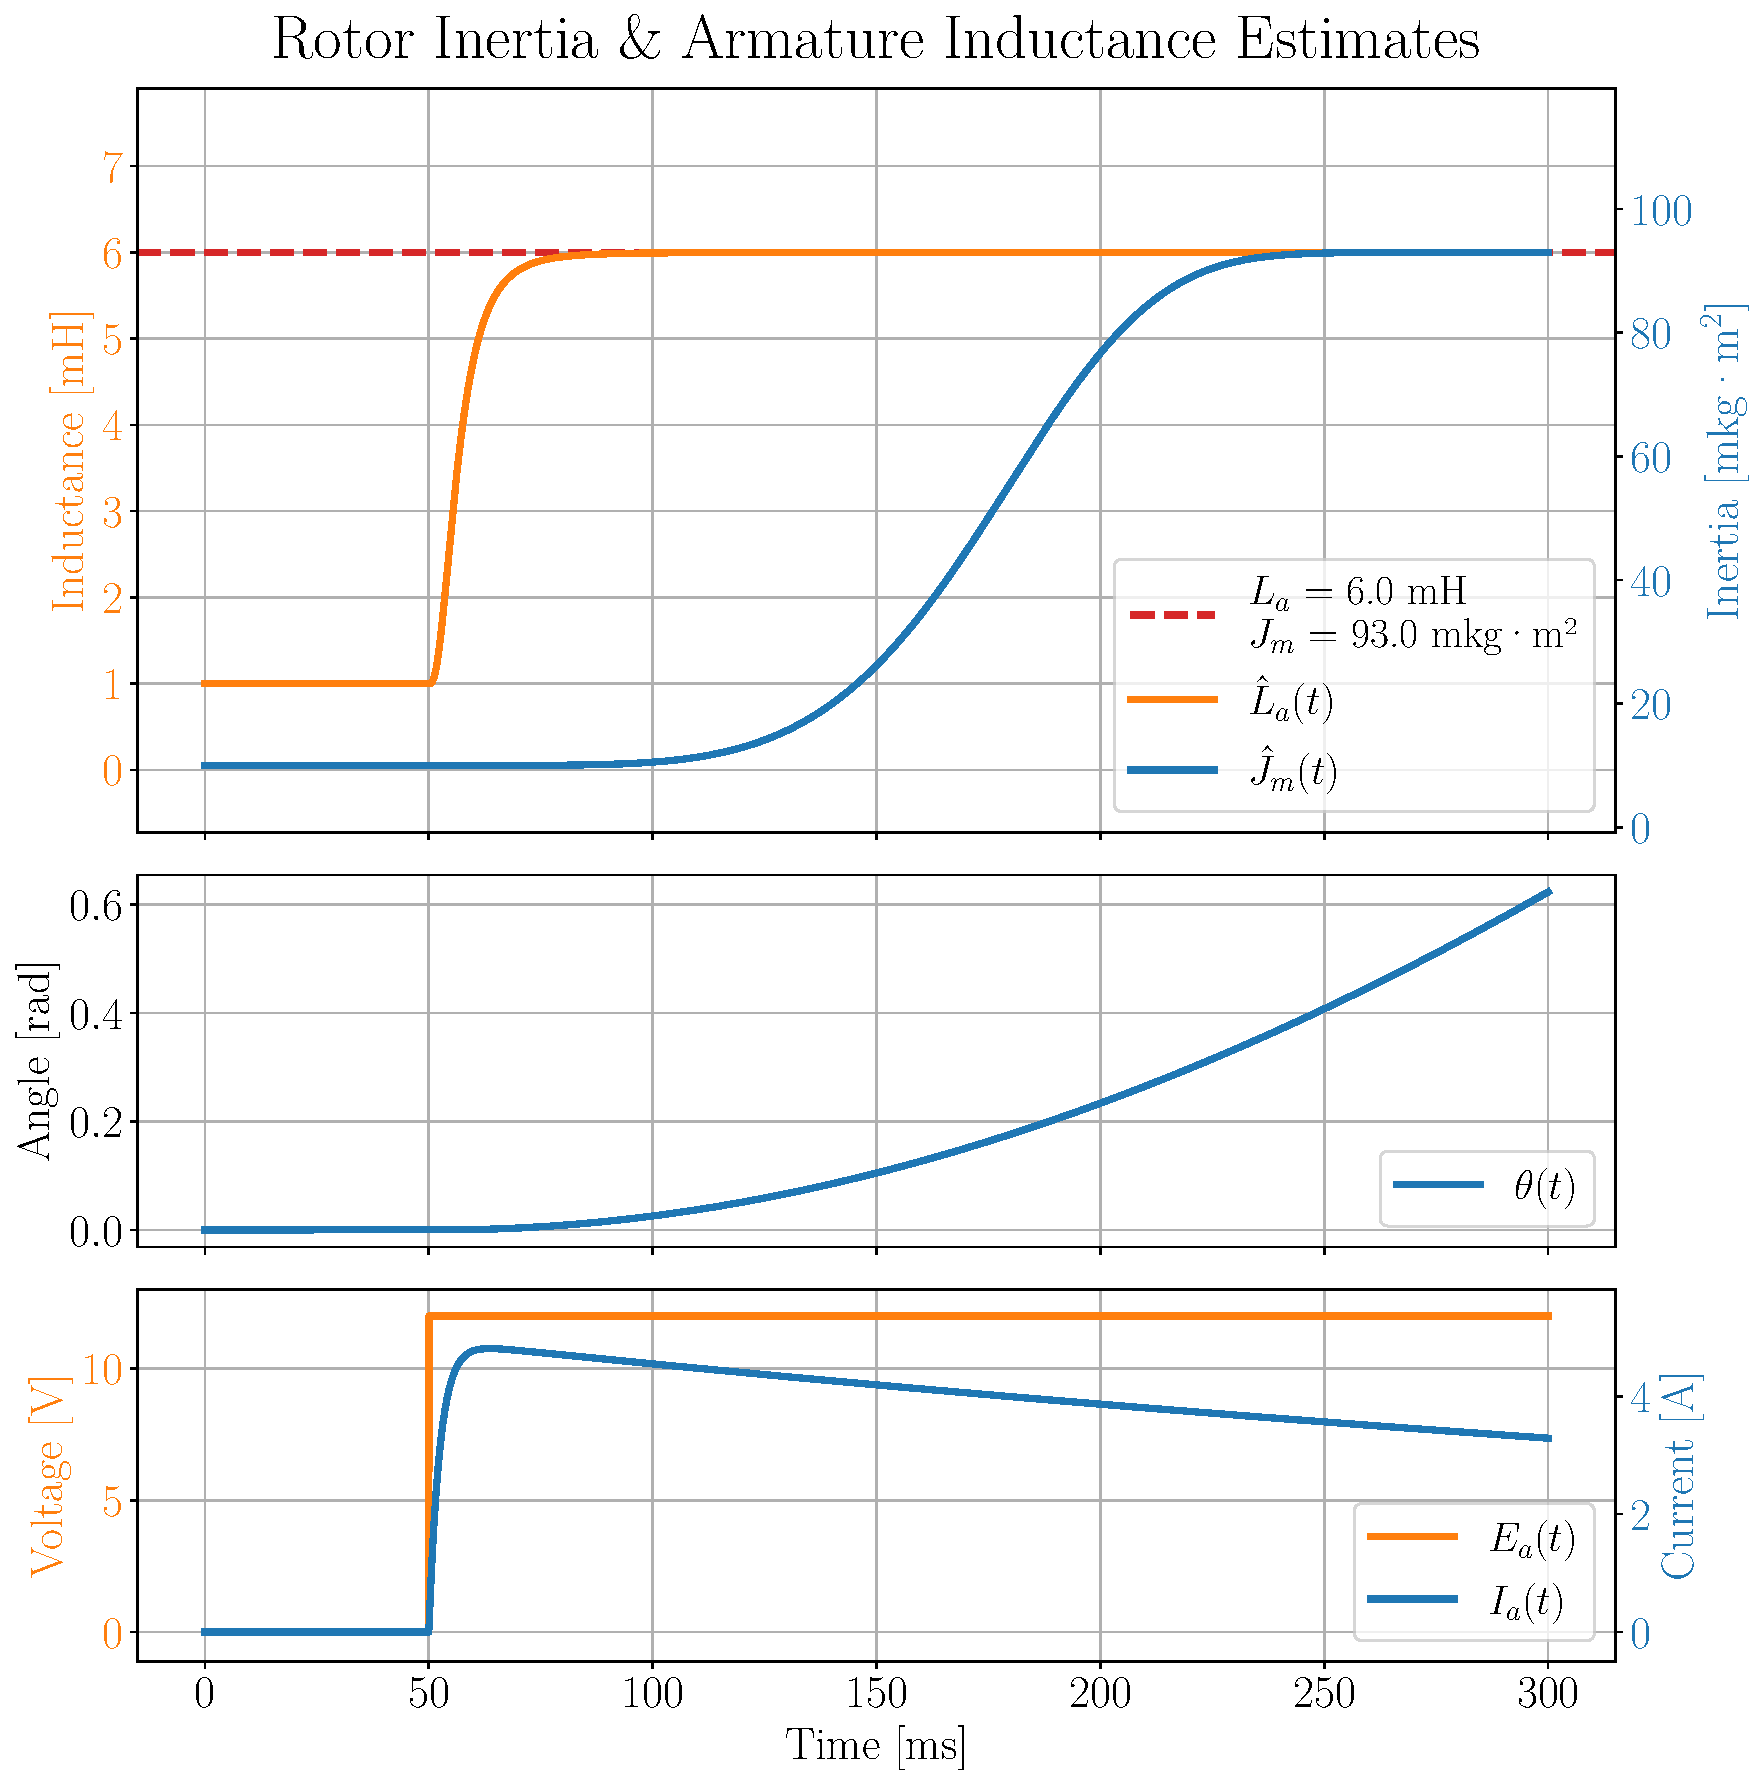
\includegraphics[width=0.8\textwidth]{../Figures/Modelling/inertia_and_inductance_estimator_gradient_results.pdf}
    \caption{Parameter identification of the armature inductance $L_a$ and rotor inertia $J_m$ using a step input in the armature voltage $E_a$.}
\end{figure}

\subsection{Mass-spring-damper load}%
\label{subsec:mass_spring_model}

In \cref{sec:finger_model} we assumed that the finger could be modelled as several torsional mass-spring-damper systems. Since we can't measure the finger-angles, in addition to that the configuration of the whiffle tree is unkown, the full finger model isn't observable, and can't be used for position control design. Instead, we'll assume that finger can be modelled as a single mass-spring-damper system, acting on the motor as $\tau_l$. This is a simplification, but it allows for a better analysis of the system. Hence we'll model the load torque $\tau_l$ as:

\begin{equation}
    \tau_l = J \frac{\mathrm{d}^2\theta}{\mathrm{d}t^2} + c \frac{\mathrm{d}\theta}{\mathrm{d}t} + k (\theta - \theta_{eq}),
\end{equation}

where $J$ is the 'total' inertia of the finger, $c$ is the 'total' damping coefficient of the finger, $k$ is the 'total' stiffness of the finger, and $\theta_{eq}$ is a kind of equilibrium angle of the finger. Substituting this into \cref{eq:motor_model_mechanical_rewrite}, we get the updated mechanical dynamics:

\begin{equation}
    \label{eq:motor_model_mechanical_load}
    (J_m + J) \frac{\mathrm{d}^2\theta}{\mathrm{d}t^2} + (B_m + c) \frac{\mathrm{d}\theta}{\mathrm{d}t} + k \theta = K_t I_a + k \theta_{eq}
\end{equation}

\subsection{State-space model of brushed DC motor with load}%
\label{subsec:state_space_model_load}

To analyze the position controller for the motor with load, discussed further in \cref{sec:mrac_implementation}, we need to express the dynamics in \cref{eq:motor_model_mechanical_load} in state-space representation, as shown in \cref{subsec:theory_control_state_space}. Assuming that $I_a$ can be treated as an input, explained in \cref{sec:controller_design_current_controller}, and defining $\omega\triangleq\frac{\mathrm{d}\theta}{\mathrm{d}t}$, we can rewrite the \cref{eq:motor_model_mechanical_load} and as:

\begin{equation}
    \frac{\mathrm{d}\omega}{\mathrm{d}t} = \frac{1}{J_m + J} \left(K_t I_a - (B_m + c) \omega - k (\theta - \theta_{eq})\right).
\end{equation}

Written in state-space form, we have:

\begin{equation}
    \label{eq:state_space_model}
    \underbrace{
    \frac{\mathrm{d}}{\mathrm{d}t}
    \begin{bmatrix}
        \theta\\
        \omega
    \end{bmatrix}}_{\textstyle \frac{\mathrm{d}}{dt}\mathbf{x}} =
    \underbrace{
    \begin{bmatrix}
        0 & 1 \\
        -\frac{k}{J_m + J} & -\frac{B_m + c}{J_m + J}
    \end{bmatrix}}_{\textstyle \mathbf{A}}
    \underbrace{
    \begin{bmatrix}
        \theta\\
        \omega
    \end{bmatrix}}_{\textstyle \mathbf{x}} +
    \underbrace{
    \begin{bmatrix}
        0\\
        \frac{K_t}{J_m + J}
    \end{bmatrix}}_{\textstyle \mathbf{B}} \underbrace{I_a}_{\textstyle \mathbf{u}} + 
    \underbrace{
    \begin{bmatrix}
        0\\
        \frac{k \theta_{eq}}{J_m + J}
    \end{bmatrix}}_{\textstyle \mathbf{d}}
\end{equation}

\begin{equation*}
    \implies \frac{\mathrm{d}}{\mathrm{d}t}\mathbf{x} = \mathbf{A}\mathbf{x} + \mathbf{B}\mathbf{u} + \mathbf{d}.
\end{equation*}

In addition we have an encoder measuring $\theta$. Hence the output of the system is given by:

\begin{equation}
    \label{eq:output_equation}
    \begin{aligned}
        \underbrace{
    \begin{bmatrix}
        \theta
    \end{bmatrix}}_{\textstyle \mathbf{y}} &=
    \underbrace{
    \begin{bmatrix}
        1 & 0
    \end{bmatrix}}_{\textstyle \mathbf{C}}
    \underbrace{
    \begin{bmatrix}
        \theta \\
        \omega
    \end{bmatrix}}_{\textstyle \mathbf{x}} \\
    \implies \mathbf{y} &= \mathbf{C}\mathbf{x}.
    \end{aligned}
\end{equation}
